\section{CPLD原理及结构}

\begin{frame}{CPLD原理及结构}
\begin{block}{复杂可编程逻辑器件(CPLD)概述}
\begin{itemize}
\tightlist
\item
    \textbf{结构}:

    \begin{itemize}
    \tightlist
    \item
    CPLD 由多个类似 SPLD 的块集成在单个芯片上组成。
    \item
    与 SPLD 相比,CPLD 更加复杂,甚至在其基本类似 SPLD
    的块级别也是如此。
    \end{itemize}
\item
    \textbf{讨论重点}:

    \begin{itemize}
    \tightlist
    \item
    \textbf{商用产品概述}:

    \begin{itemize}
    \tightlist
    \item
        首先对市场上的商用 CPLD 产品进行详细讨论。
    \end{itemize}
    \item
    \textbf{适用应用}:

    \begin{itemize}
    \tightlist
    \item
        探讨 CPLD 最适合的应用类型。
    \end{itemize}
    \item
    \textbf{产品比较}:

    \begin{itemize}
    \tightlist
    \item
        提供足够的细节,便于比较各种竞争产品。
    \item
        特别关注使用更广泛的器件。
    \end{itemize}
    \end{itemize}
\end{itemize}
\end{block}
\end{frame}

\subsection{Altera CPLD}
\begin{frame}[allowframebreaks]{\textbf{Altera CPLD 产品系列}}
    \begin{itemize}
    \tightlist
    \item
    Altera 开发了三类属于 CPLD 的芯片系列:MAX 5000、MAX 7000 和 MAX
    9000。
    \item
    \textbf{MAX 7000 系列}:

    \begin{itemize}
    \tightlist
    \item
        广泛使用,提供先进的逻辑容量和速度性能。
    \item
        是讨论的重点。
    \end{itemize}
    \item
    \textbf{MAX 5000 系列}:

    \begin{itemize}
    \tightlist
    \item
        代表了一种较旧的技术,提供成本效益高的解决方案。
    \end{itemize}
    \item
    \textbf{MAX 9000 系列}:

    \begin{itemize}
    \tightlist
    \item
        与 MAX 7000 类似,但提供更高的逻辑容量(业界最高)。
    \end{itemize}
    \end{itemize}
\end{frame}

\begin{frame}[allowframebreaks]{MAX7000系列架构}:

    \begin{itemize}
    \tightlist
    \item
    \begin{figure}
        \centering
        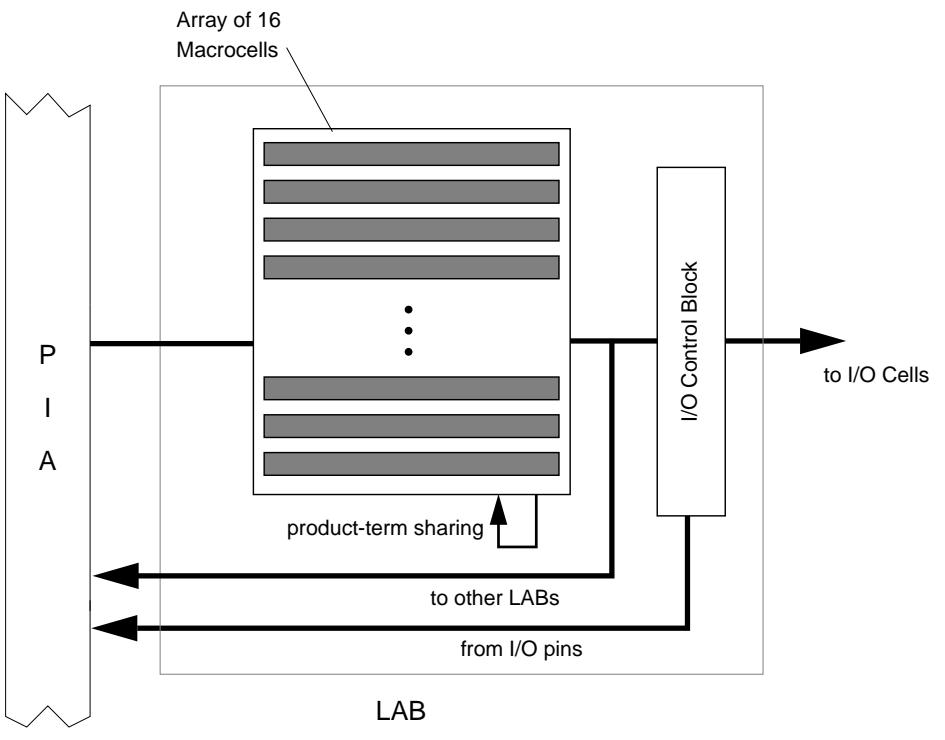
\includegraphics[width=0.55\textwidth,keepaspectratio]{img1/MAX7000.jpeg}
        \caption{Altera MAX7000的逻辑阵列模块}
    \end{figure}

    如图所示,由以下部分组成:
    \begin{itemize}
    \tightlist
    \item
        \textbf{Logic Array Blocks (LABs)}: 逻辑阵列块。
    \item
        \textbf{Programmable Interconnect Array (PIA)}:
        可编程互连阵列,能够连接任何 LAB 的输入或输出。
    \end{itemize}
    \item
    芯片的输入和输出直接连接到 PIA 和 LABs。
    \item
    LAB 可以被视为一种复杂的 SPLD 结构,因此整个芯片可以看作是一个 SPLD
    阵列。
    \item
    \textbf{编程技术}:

    \begin{itemize}
    \tightlist
    \item
        MAX 7000 器件基于 EPROM 和 EEPROM 技术。
    \item
        1996 年,Altera 发布了 7000S 系列,支持``电路内''可重复编程。
    \end{itemize}
    \end{itemize}
\end{frame}

\begin{frame}[allowframebreaks]{\textbf{LAB 结构}}

    \begin{figure}
    \centering
    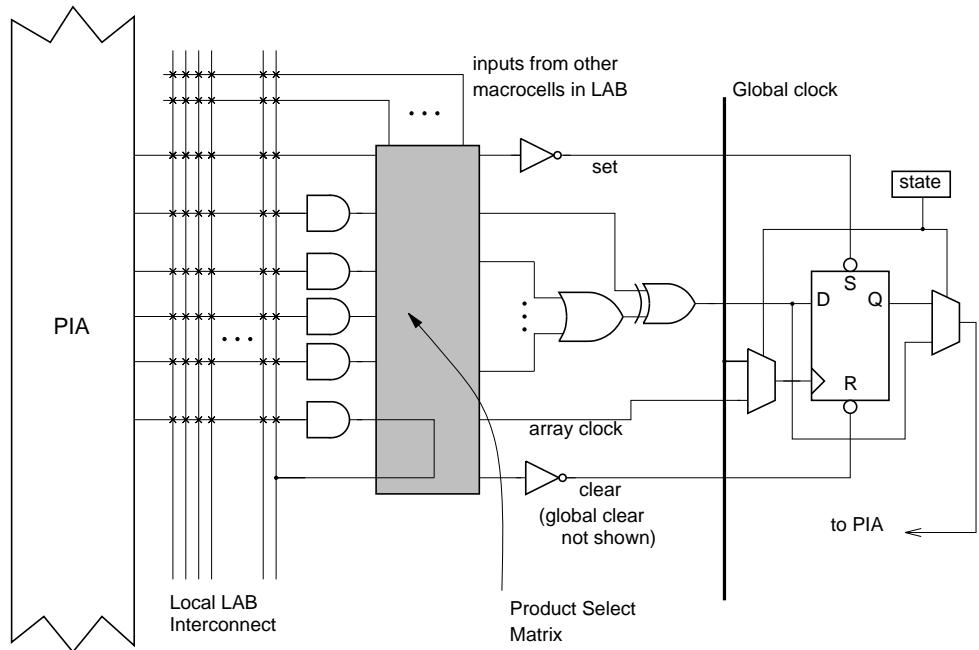
\includegraphics[width=0.6\textwidth]{img1/MAX7000Macrocell.jpeg}
    \caption{MAX7000宏单元}
    \end{figure}

    \begin{itemize}
    \tightlist
    \item
    每个 LAB 由两组八个\textbf{宏单元}组成。
    \item
    \textbf{宏单元}:

    \begin{itemize}
    \tightlist
    \item
        包含一组可编程乘积项(与门平面的一部分),驱动或门和触发器。
    \item
        触发器可配置为 D 型、JK、T、SR 或透明。
    \end{itemize}
    \item
    \textbf{或门输入}:

    \begin{itemize}
    \tightlist
    \item
        或门的输入数量可变,可以来自宏单元内的最多五个乘积项,还可以从同一
        LAB 内的其他宏单元引入最多15个额外的乘积项。
    \item
        这种灵活性使得 MAX 7000 系列在芯片面积利用上更加高效。
    \end{itemize}
    \end{itemize}
\end{frame}

\subsection{AMD Mach 系列 CPLD}
\begin{frame}[allowframebreaks]{\textbf{AMD Mach CPLD产品系列}}
    \begin{itemize}
    \tightlist
    \item
    AMD 提供五个子系列的 CPLD,称为 Mach 1 到 Mach 5。
    \item
    每个 Mach 器件由多个类似 PAL 的块组成:

    \begin{itemize}
    \tightlist
    \item
        \textbf{Mach 1 和 Mach 2}: 由优化的 22V16 PAL 构成。
    \item
        \textbf{Mach 3 和 Mach 4}: 由多个优化的 34V16 PAL 构成。
    \item
        \textbf{Mach 5}: 结构类似,但提供增强的速度性能。
    \end{itemize}
    \item
    \textbf{编程技术}: 所有 Mach 芯片都基于 EEPROM 技术。
    \item
    \textbf{产品范围}:
    五个子系列提供了广泛的选择,从小型、低成本的芯片到大型、先进的芯片。
    \item
    \textbf{讨论重点}: Mach 4 系列,因为它代表了 Mach
    家族中最先进的产品。
    \end{itemize}
\end{frame}

\begin{frame}[allowframebreaks]{\textbf{Mach 4 架构}}

    \begin{itemize}
    \tightlist
    \item
    Mach 4 芯片由多个 34V16 类似 PAL的块组成,并通过中央交换矩阵(Central Switch Matrix)互连。
    \item
    \textbf{芯片规模}: 从 6 到 16 个 PAL 块不等,对应的等效门数约为 2000
    到 5000。
    \item
    \textbf{编程方式}: 支持电路内编程。
    \item
    \textbf{互连方式}: 所有 PAL
    块之间的连接(包括块内部连接)都通过中央交换矩阵进行。
    \item
    \textbf{延迟特性}: 由于所有连接都通过相同的路径,Mach 4
    实现的电路时序延迟是可预测的。
    \end{itemize}

\begin{figure}
    \centering
    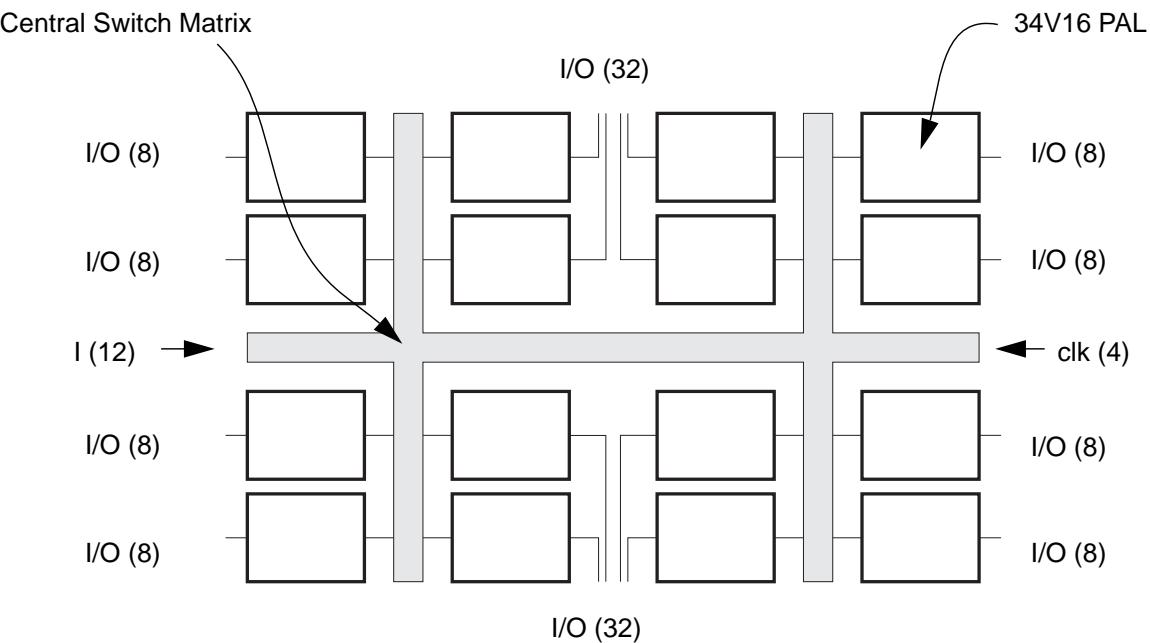
\includegraphics[width=0.7\textwidth]{img1/MAch4.jpeg}
    \caption{Mach 4 CPLD结构}
\end{figure}
\end{frame}

\begin{frame}{\textbf{Mach 4 PAL 块结构}}

    \begin{itemize}
    \tightlist
    \item
    每个类似 PAL 的块具有 16 个输出和 34 个输入(其中 16
    个为反馈输出),相当于一个 34V16 PAL。
    \item
    \textbf{关键改进}:

    \begin{enumerate}
    \tightlist
    \item
        \textbf{乘积项分配器(Product Term Allocator)}:
        位于与门平面和宏单元之间,负责将与门平面的乘积项分配给需要的或门。
    \item
        \textbf{输出交换矩阵(Output Switch Matrix)}: 位于或门和 I/O
        引脚之间,允许任何宏单元输出驱动连接到 PAL 块的任何 I/O 引脚。
    \end{enumerate}
    \item
    \textbf{灵活性}:

    \begin{itemize}
    \tightlist
    \item
        乘积项分配器使得与门平面的乘积项可以在或门之间灵活共享。
    \item
        输出交换矩阵增强了引脚分配的灵活性。
    \end{itemize}
    \item
    \textbf{优点}: 系统内编程和高灵活性使得硬件设计变更更加容易。
    \end{itemize}
\end{frame}

\subsection{Lattice CPLD}
\begin{frame}[allowframebreaks]{\textbf{Lattice CPLD 产品系列}}
\begin{itemize}
\tightlist
\item
    \textbf{产品系列}:

    \begin{itemize}
    \tightlist
    \item
    Lattice 提供完整的 CPLD 产品线,主要包括两类产品:

    \begin{itemize}
    \tightlist
    \item
        \textbf{pLSI}: 三个系列的 EEPROM 型 CPLD。
    \item
        \textbf{ispLSI}: 与 pLSI 相同,但支持系统内编程(in-system
        programmable)。
    \end{itemize}
    \item
    \textbf{产品家族}:

    \begin{itemize}
    \tightlist
    \item
        每个系列(pLSI 和 ispLSI)都提供三种不同逻辑容量和速度性能的产品。
    \end{itemize}
    \end{itemize}
\item
    \textbf{1000 系列}:

    \begin{itemize}
    \tightlist
    \item
    \textbf{逻辑容量}: 约 1200 到 4000 门。
    \item
    \textbf{引脚到引脚延迟}: 10 纳秒。
    \item
    \textbf{结构}:

    \begin{itemize}
    \tightlist
    \item
        由多个类似 SPLD 的块组成,通过全局路由池(Global Routing Pool,
        GRP)连接。
    \end{itemize}
    \end{itemize}
\item
    \textbf{2000 系列}:

    \begin{itemize}
    \tightlist
    \item
    \textbf{逻辑容量}: 600 到 2000 门。
    \item
    \textbf{特点}:

    \begin{itemize}
    \tightlist
    \item
        宏单元与 I/O 引脚的比率更高。
    \item
        速度性能优于 1000 系列。
    \end{itemize}
    \item
    \textbf{引脚到引脚延迟}: 5.5 纳秒,提供业界领先的速度。
    \end{itemize}
\item
    \textbf{3000 系列}:

    \begin{itemize}
    \tightlist
    \item
    \textbf{逻辑容量}: 高达 5000 门。
    \item
    \textbf{引脚到引脚延迟}: 约 10-15 纳秒。
    \item
    \textbf{功能}:

    \begin{itemize}
    \tightlist
    \item
        与 AMD Mach 4 相似。
    \item
        提供额外的增强功能,支持 JTAG 边界扫描等现代设计风格。
    \end{itemize}
    \end{itemize}
\end{itemize}
\end{frame}

\begin{frame}[allowframebreaks]{\textbf{Lattice pLSI/ispLSI 结构}}
    \begin{itemize}
    \tightlist
    \item
    芯片外边缘是双向
    I/O,直接连接到\textbf{通用逻辑块(Generic Logic Blocks,
    GLBs)}和\textbf{全局路由池(GRP)}。
    \item
    \textbf{GLBs}:

    \begin{itemize}
    \tightlist
    \item
        类似 PAL 的小块,包含与门平面、乘积项分配器和宏单元。
    \end{itemize}
    \item
    \textbf{GRP}:

    \begin{itemize}
    \tightlist
    \item
        一组跨越整个芯片的导线,用于连接 GLB 的输入和输出。
    \item
        所有互连都通过 GRP 进行,因此Lattice芯片的时序完全可预测,类似于
        AMD Mach 器件。
    \end{itemize}
\end{itemize}
\pagebreak
\begin{figure}
    \centering
    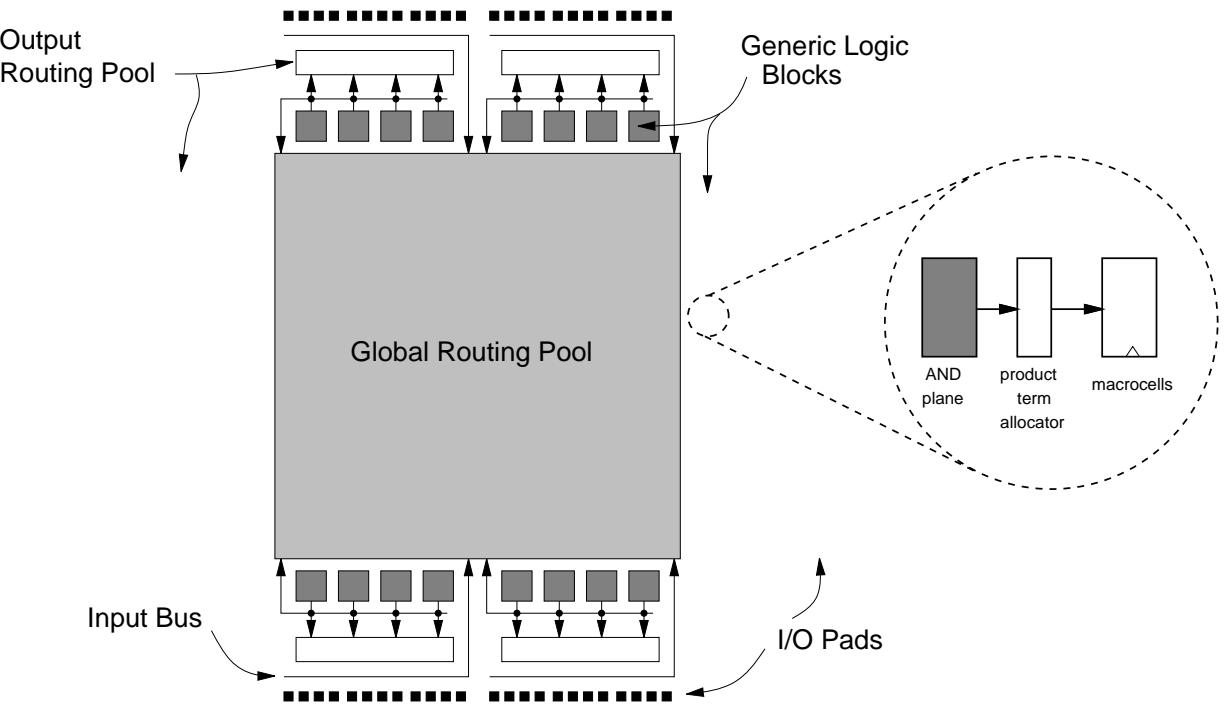
\includegraphics[width=0.8\textwidth]{img1/lattice.jpeg}
    \caption{Lattice (i)PLSI 架构图.}
\end{figure}

\end{frame}


\subsection{Cypress CPLD}
\begin{frame}[allowframebreaks]{\textbf{Cypress CPLDs的特点}}
\begin{itemize}
\tightlist
\item
    \textbf{技术基础}:

    \begin{itemize}
    \tightlist
    \item
    Cypress 最近开发了一类 CPLD 产品,称为 FLASH370,基于 FLASH EEPROM
    技术。
    \item
    在多个方面与 AMD 和 Lattice 的器件类似。
    \end{itemize}
\item
    \textbf{性能}:

    \begin{itemize}
    \tightlist
    \item
    \textbf{引脚到引脚延迟}: 8.5 到 15 纳秒。
    \item
    \textbf{编程方式}: 不支持系统内编程。
    \end{itemize}
\item
    \textbf{I/O 特点}:

    \begin{itemize}
    \tightlist
    \item
    较大的芯片需要更多的 I/O,因此 FLASH370 提供了比竞争产品更多的 I/O。
    \item
    宏单元数量与双向 I/O 引脚数量呈线性关系:

    \begin{itemize}
    \tightlist
    \item
        最小器件:32 宏单元和 32 I/O。
    \item
        最大器件:256 宏单元和 256 I/O。
    \end{itemize}
    \end{itemize}
\end{itemize}
\end{frame}

\begin{frame}[allowframebreaks]{\textbf{FLASH370 架构}}
    \begin{itemize}
    \tightlist
    \item
    FLASH370 具有典型的 CPLD 架构:

    \begin{itemize}
    \tightlist
    \item
        多个类似 PAL 的块。
    \item
        可编程互连矩阵(Programmable Interconnect Matrix,
        PIM)用于连接这些块。
    \end{itemize}
    \item
    \textbf{PAL 块内部结构}:

    \begin{itemize}
    \tightlist
    \item
        \textbf{与门平面(AND-plane)}: 驱动乘积项分配器。
    \item
        \textbf{乘积项分配器}: 将 0 到 16
        个乘积项分配给每个或门(共32个)。
    \item
        \textbf{反馈路径}: 从宏单元输出到 PIM 有 32
        条导线,允许宏单元被``埋入''(不驱动 I/O 引脚),同时仍可将 I/O
        引脚用作输入。   
    \end{itemize}
    \end{itemize}

\begin{figure}
    \centering
    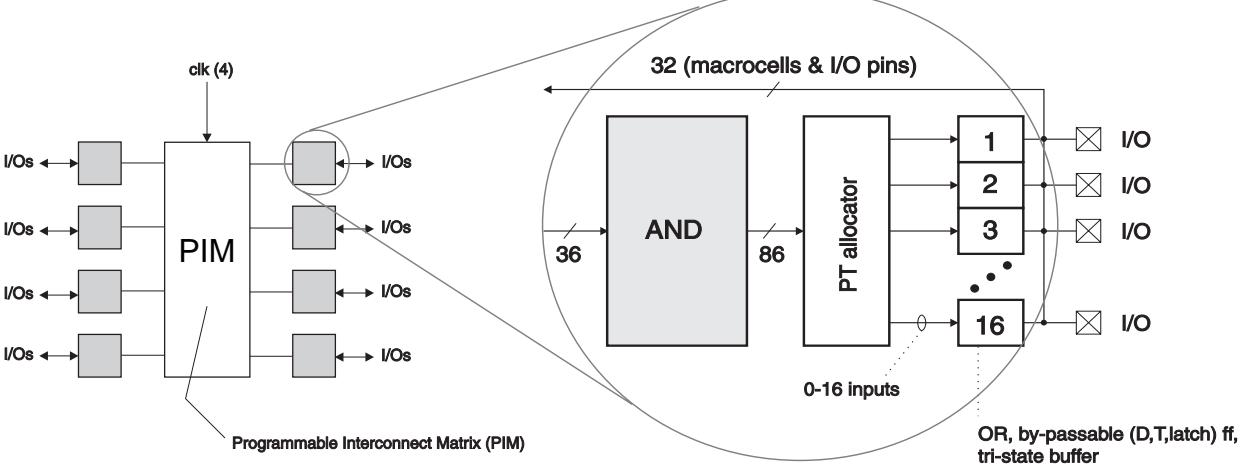
\includegraphics[width=0.8\textwidth]{img1/cypress.jpeg}
    \caption{Cypress FLASH370 CPLD架构图.}
\end{figure}
CPLD 中类似 PAL 的块提供了额外灵活性,这是普通 PAL 所不具备的。
\end{frame}


\subsection{Xilinx CPLD}
\begin{frame}[allowframebreaks]{\textbf{Xilinx XC7000 CPLDs}}
\phantomsection\label{xilinx-xc7000-cplds}
\begin{itemize}
\tightlist
\item
    \textbf{概述}:

    \begin{itemize}
    \tightlist
    \item
    Xilinx 主要生产 FPGA,但也提供一系列 CPLD,称为 XC7000,并宣布了新的
    CPLD 系列 XC9500。
    \item
    XC7000 系列包括两个主要家族:7200 系列和 7300 系列。
    \end{itemize}
\item
    \textbf{7200 系列}:

    \begin{itemize}
    \tightlist
    \item
    \textbf{来源}: 最初由 Plus Logic 作为 Hiper EPLDs 推向市场。
    \item
    \textbf{逻辑容量}: 约 600 到 1500 门。
    \item
    \textbf{速度性能}: 引脚到引脚延迟约为 25 纳秒。
    \item
    \textbf{结构}:

    \begin{itemize}
    \tightlist
    \item
        由多个类似 SPLD 的块组成,每个块包含 9 个宏单元。
    \end{itemize}
    \item
    \textbf{宏单元特点}:

    \begin{itemize}
    \tightlist
    \item
        每个宏单元包含两个或门。
    \item
        每个或门的输入连接到一个两位算术逻辑单元(ALU)。
    \item
        ALU
        可以生成其两个输入的任何函数,并将其输出馈送到可配置的触发器中。
    \end{itemize}
    \end{itemize}
\item
    \textbf{7300 系列}:

    \begin{itemize}
    \tightlist
    \item
    \textbf{特点}: 是 7200 系列的增强版本。
    \item
    \textbf{逻辑容量}: 高达 3000 门(当整个系列可用时)。
    \item
    \textbf{速度性能}: 更高的速度性能。
    \end{itemize}
\item
    \textbf{XC9500 系列}:

    \begin{itemize}
    \tightlist
    \item
    \textbf{特点}:

    \begin{itemize}
    \tightlist
    \item
        支持系统内编程。
    \item
        引脚到引脚延迟为 5 纳秒。
    \item
        逻辑容量高达 6200 门。
    \end{itemize}
    \end{itemize}
\end{itemize}
\end{frame}

\subsection{CPLD的应用}
\begin{frame}[allowframebreaks]{\textbf{CPLD 的应用}}
\phantomsection\label{cpld-ux7684ux5e94ux7528}
\begin{itemize}
\tightlist
\item
    \textbf{概述}:

    \begin{itemize}
    \tightlist
    \item
    CPLD
    因其高速度和广泛的容量范围,适用于多种应用,从实现随机粘合逻辑到小型门阵列的原型设计。
    \item
    目前工业中最常见的用途之一是将多个 SPLD 的设计转换为更少数量的
    CPLD,这是 CPLD 市场快速增长的重要原因。
    \end{itemize}
\item
    \textbf{具体应用}:

    \begin{itemize}
    \tightlist
    \item
    \textbf{复杂设计实现}:

    \begin{itemize}
    \tightlist
    \item
        如图形控制器、LAN 控制器、UARTs、缓存控制等。
    \end{itemize}
    \item
    \textbf{适合的电路类型}:

    \begin{itemize}
    \tightlist
    \item
        能够利用宽与门/或门且不需要大量触发器的电路非常适合在 CPLD
        中实现。
    \end{itemize}
    \end{itemize}
\item
    \textbf{设计优势}:

    \begin{itemize}
    \tightlist
    \item
    \textbf{可重复编程}:

    \begin{itemize}
    \tightlist
    \item
        所有商用 CPLD 产品都支持重新编程,简化了设计变更。
    \end{itemize}
    \item
    \textbf{系统内编程}:

    \begin{itemize}
    \tightlist
    \item
        支持在不停机的情况下重新配置硬件(例如更改通信电路的协议)。
    \end{itemize}
    \end{itemize}
\item
    \textbf{设计分区与性能预测}:

    \begin{itemize}
    \tightlist
    \item
    设计通常自然地划分为 CPLD 中类似 SPLD 的块。
    \item
    这种分区的结果是比将设计分割成许多小部分并将其映射到芯片不同区域更可预测的速度性能。
    \item
    \textbf{电路实现的预测性}:

    \begin{itemize}
    \tightlist
    \item
        这是 CPLD 架构最显著的优势之一。
    \end{itemize}
    \end{itemize}
\end{itemize}
\end{frame}
